\chapter{Mesh Data Structure}
\label{chap:meshds}

Let $\Omega$ be a three-dimensional domain with boundary $\partial\Omega$. A tetrahedral mesh of $\Omega$ is a three-dimensional simplicial complex ${\cal T}$. It contains a subcomplex ${\cal F}$ which is the surface mesh of $\partial\Omega$. ${\cal F}$ a two-dimensional simplicial complex.

For storing and maintaining a tetrahedral mesh ${\cal T}$ as well as its subcomplex ${\cal F}$, we use the following lists of elements:
\begin{itemize}
\item a list of vertices of ${\cal T}$;
\item a list of tetrahedra of ${\cal T}$;
\item a list of subfaces of ${\cal F}$; and
\item a list of subsegment of ${\cal F}$.
\end{itemize}
Where subfaces and subsegments are those faces and edges belong to both ${\cal T}$ and {\cal F}, respectively. Since we store all tetrahedra, there is no need to store faces and edges of ${\cal T}$. While subfaces and subsegments are stored explicitly. 

\section{Basic Mesh Data Types}

There are four types of mesh elements: vertices, tetrahedra, subfaces, and subsegments. The elements of all the four types consist of a tetrahedral mesh of a 3D domain.  Three data structures are declared:  {\it tetrahedron}, {\it shellface}, and {\it point}. A tetrahedron is a tetrahedron;  a shellface can be either a subface or a subsegment;  and a point is a point. These three data types, linked by pointers comprise a mesh.

\subsection{Point}

The {\it point} data structure is a list of floating-point numbers. This list contains the following data of the point:
\begin{itemize}
\item $3$ coordinates;
\item $n$ user-defined attributes (optional);
\item $1$ user-defined metric tensor (optional);
\item $1$ pointer to a simplex (tet, tri, edge); 
\item $1$ pointer to a parent (or duplicate) point;
\item $1$ pointer to a tet in background mesh (optional);
\item $1$ integer index (also for boundary marker);
\item $1$ integer for the vertex type.
\end{itemize}

\subsection{Shellface}

The {\it shellface} data structure represents either a subface or a subsegment. It contains the following data (see Fig.~\ref{fig:shellface-tetrahedron} left):
\begin{itemize}
\item $3$ pointers to adjacent subfaces;
\item $3$ pointers to its points;
\item $2$ pointers to adjacent tetrahedra;
\item $3$ pointers to adjacent subsegments;
\item $1$ pointer to a badface (optional);
\item $1$ double of maximum area (optional);
\item $1$ integer of boundary marker;
\item $1$ integer of type;
\end{itemize}

Fig.~\ref{fig:shellface} shows a subface with its adjacent subfaces, subsegments, and tetrahedra. Note that the three adjacent subsegments is not always exist, if so, they are set to {\tt dummysh}). 

\begin{figure}
  \centering
  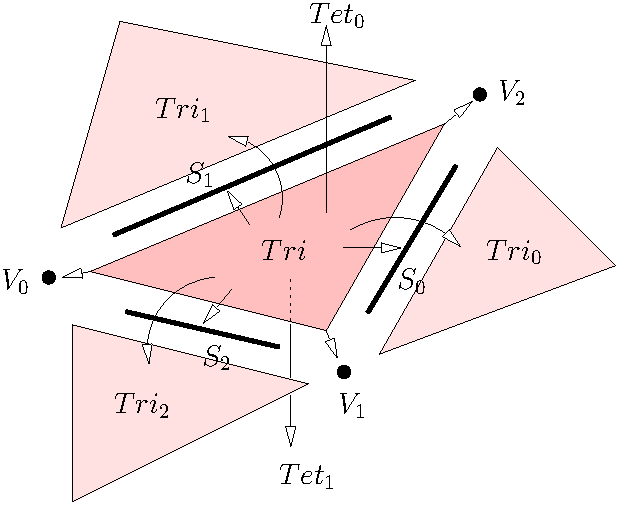
\includegraphics[width=0.6\textwidth]{../figs/triang-edge-ds}
\caption{The shellface data structures.}
\label{fig:shellface}
\end{figure}

Note that a shellface is also used to store a subsegment. In such case, the third point of it is set to {\tt null}. And it has only one pointer to an adjacent subface.  Since there may be arbitrary number of subfaces containing a subsegment, chose one arbitrarily.

\subsection{Tetrahedron}

The {\it tetrahedron} data structure represent a tetrahedron. It contains the following data (see Fig.~\ref{fig:tetrahedron} right):
\begin{itemize}
\item $4$ pointers to adjacent tetrahedron;
\item $4$ pointers to its points;
\item $4$ pointers to adjacent subfaces (optional, -p, -r options);
\item $2$ pointers to adjacent subsegments (optional, -p, -r options);
\item $n$ user-defined attributes (optional);
\item $1$ double of maximum volume (optional);
\item $1$ pointer to a list of higher order nodes (-o2 option);
\end{itemize}

\begin{figure}
  \centering
  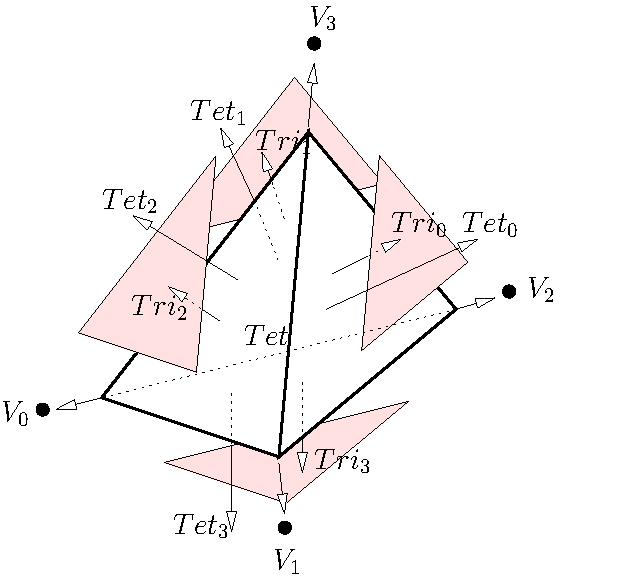
\includegraphics[width=0.8\textwidth]{../figs/tetrahedron-based}
\caption{The tetrahedron data structures.}
\label{fig:tetrahedron}
\end{figure}

\section{Mesh Handles}

Two special data types, 'triface' and 'face' are defined for maintaining and updating meshes. They are like pointers (or handles), which allow you to hold one particular part of the mesh, i.e., a tetrahedron, a triangle, an edge and a vertex.  However, these data types do not themselves store any part of the mesh. The mesh is made of the data types defined above.

\subsection{Face}

Let the three vertices of a triangle be ordered and numbered as $v_0$, $v_1$, and $v_2$. The six versions of the directed edges $(i, j)$ of this triangle (see Fig.~\ref{fig:edge-versions}) are defined as follows:\\
\begin{tabular}{rl}
$0$ & $(v_0, v_1)$\\
$1$ & $(v_1, v_0)$\\
$2$ & $(v_1, v_2)$\\
$3$ & $(v_2, v_1)$\\
$4$ & $(v_2, v_0)$\\
$5$ & $(v_0, v_2)$
\end{tabular}\\
The {\it face} handle holds a directed edge of a shellface. A set of mesh manipulation primitives are defined for various operation on faces.

\begin{figure}
  \centering
  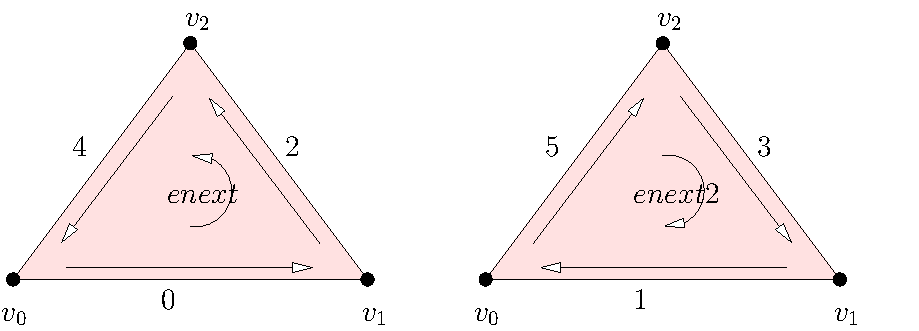
\includegraphics[width=1.0\textwidth]{../figs/face-versions}
\caption{The six versions of the directed edges of a triangle.}
\label{fig:edge-versions}
\end{figure}

\subsection{Triface}

Let the four nodes of a tetrahedron be ordered and numbered from $v_0, ..., v_3$. The order of the nodes is chosen in such a way that the signed volume of the tetrahedron evaluated by $v_0, ..., v_3$ is negative. Intuitively, the last node ($v_3$) "sees" the first three nodes ($v_0, v_1, v_2$) in counterclockwise order. 

Let the four faces of a tetrahedron be numbered from $f_0, ..., f_3$.  Each face has $6$ directed edges (edge versions are the same as in Fig.~\ref{fig:edge-versions}). We stipulate the four faces and the directed edges in each face as in Fig.~\ref{fig:triface}.

\begin{figure}
  \centering
  \begin{tabular}{cc}
  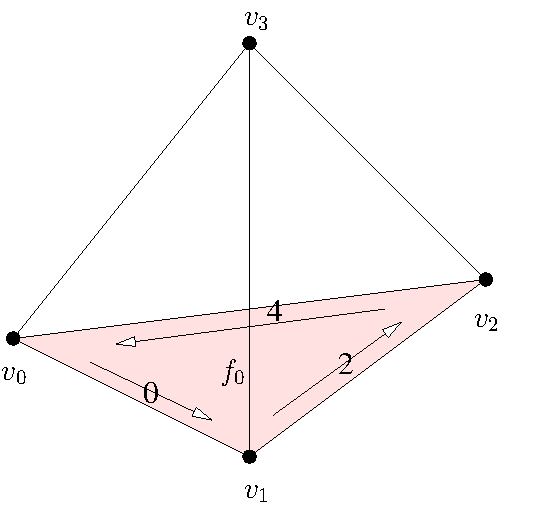
\includegraphics[width=0.45\textwidth]{../figs/triface-f0} &
  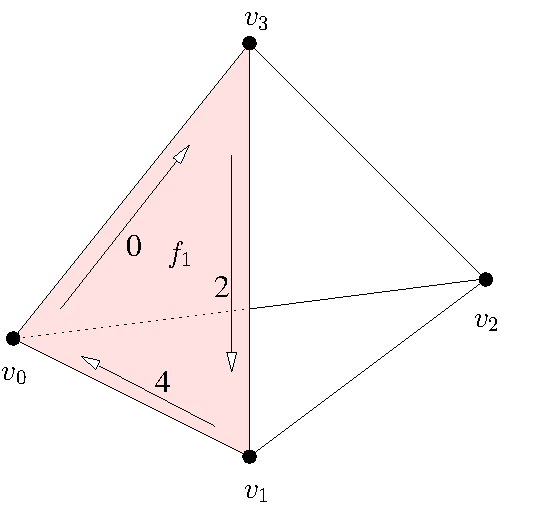
\includegraphics[width=0.45\textwidth]{../figs/triface-f1} \\
  $f_0: (v_0, v_1, v_2)$ & $f_1: (v_0, v_3, v_1)$\\
  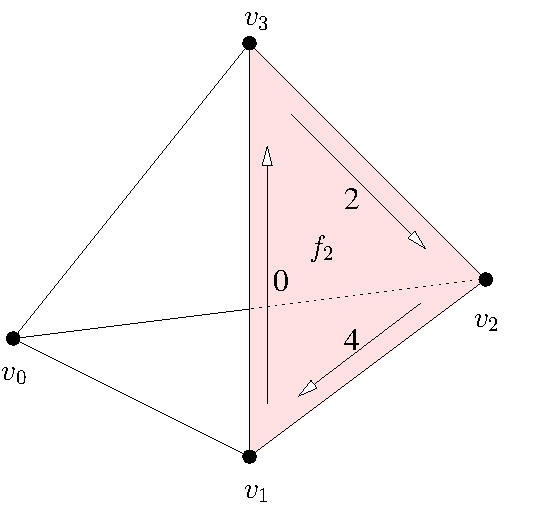
\includegraphics[width=0.45\textwidth]{../figs/triface-f2} &
  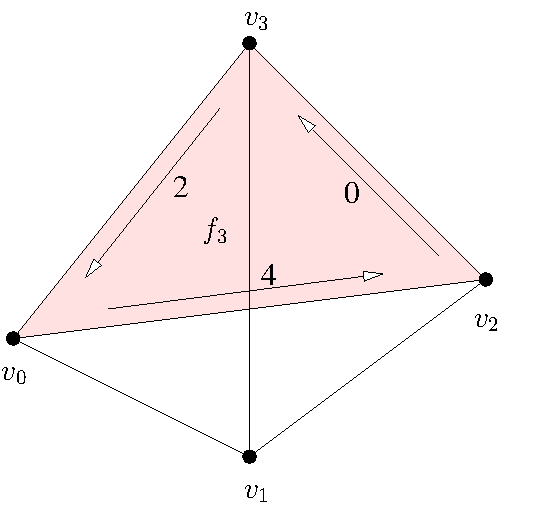
\includegraphics[width=0.45\textwidth]{../figs/triface-f3} \\
  $f_2: (v_1, v_3, v_2)$ & $f_3: (v_2, v_3, v_0)$
  \end{tabular}
\caption{The faces and directed edges of a tetrahedron.}
\label{fig:triface}
\end{figure}
 
The {\it triface} handle holds a directed edge of a terahedron. A set of mesh manipulation primitives are defined for various operation on trifaces.

\section{Primitives for Mesh Manipulations}

The mesh data structures additionally store geometric informations which help for fast queries.

\subsection{bond}

Suppose two trifaces $t_1$ and $t_2$ share the same faces. The {\tt bond} primitive connects $t_1$ and $t_2$ together. It also encodes the $0$-th edge informations of $t_1$ and $t_2$, i.e., at $t_1$ side, the edge of $t_2$ which corresponding to the $0$-th edge of $t_1$ is bonded, and vice versa at $t_2$ side.

\begin{figure}
  \centering
  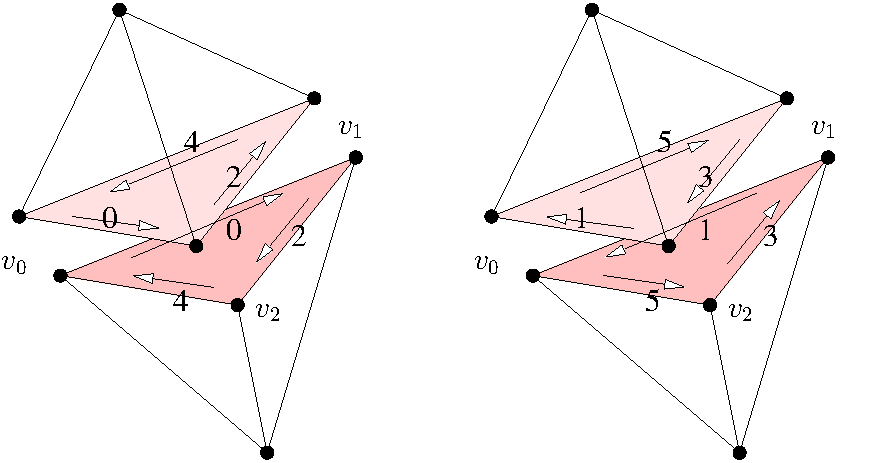
\includegraphics[width=1.0\textwidth]{../figs/fnext-base}
\caption{The {\tt bond()} and {\tt fnext()} primitives.}
\label{fig:fnext}
\end{figure}

For an example, in Fig.~\ref{fig:fnext} left, let $t_1$ be the bottom shaded face, and $t_2$ be the top shaded face. Then $t_1$ connects to the $4$-th edge of $t_2$, and $t_2$ connects the $4$-th edge of $t_1$.

\subsection{fnext}

Let $t_1$ be a triface representing the tetrahedron $(v_0, v_1, v_2, v_3)$, and $t_1$ also represents the face $(v_0, v_1, v2)$ (see Fig.~\ref{fig:fnext}), and it holds the edge $[v_0, v_1]$. The {\tt fnext} primitive returns a new triface $t_2$ such that $t_2$ holds the same edge $[v_0, v_1]$, and it represents a face $v_0, v_1, v_k]$ which is the next face in the face ring of the edge $[v_0, v_1]$, and $t_1$, $t_2$ represent different tetrahedra, respectively. 

